\section{Win32 PE}

\acs{PE} это формат исполняемых файлов, принятый в Windows.

Разница между .exe, .dll, .sys в том, что у .exe обычно нет экспортов, только импорты.

У .dll есть точка входа (\ac{OEP}), там располагается DllMain(), но обычно, эта
функция ничего не делает.

.sys это обычно драйвера устройство. Для драйверов Windows требует чтобы контрольная сумма в файле была проставлена
и была верной\footnote{Например, Hiew\ref{Hiew} умеет подсчитывать эту сумму}.
А начиная с Windows Vista, файлы-драйвера должны быть также подписаны при помощи электронной подписи, 
иначе они не будут загружаться.

\index{MS-DOS}
В начале всякого PE-файла есть небольшая DOS-программа, выводящая на консоль сообщение вроде ``This program cannot be run in DOS mode.'' --- 
это сделано для того, что если запустить эту программу в DOS либо Windows 3.1, выведется это сообщение.

\subsection{\IFRU{Терминология}{Terminology}}

\begin{itemize}
\item
Модуль --- это отдельный файл, .exe или .dll.

\item
Процесс --- это некая работающая загруженная в память и программа. Как правило состоит из одного .exe-файла и массы
.dll-файлов.

\item
Память процесса --- память с которой работает процесс. Каждого процесса --- своя. Имеются загруженные модули, память
стека, кучи (heap), итд.

\item
\ac{VA} --- это адрес, который будет использоваться в самой программе.

\item
Базовый адрес --- это адрес, по которому модуль будет загружен в пространство процесса.

\item
\ac{RVA} --- это \ac{VA}-адрес минус базовый адрес. Многие адреса в таблицах PE-файла используют именно \ac{RVA}-адреса.

\item
\ac{IAT} --- самая главная таблица описывающая импорты\footnote{\cite{Pietrek1}}.
\end{itemize}

\subsection{\IFRU{Базовый адрес}{Base address}}
Дело в том что несколько авторов могут готовить DLL-файлы для других, и нет возможности договориться о том, какие адреса и кому будут отведены.
Поэтому, если у двух необходимых для загрузки DLL одинаковые базовые адреса, одна из них будет загружена по нему, а вторая --- по другому, свободному, и все виртуальные адреса во второй DLL будут изменены. \\
\\
Очень часто, по крайней мере линкер в \ac{MSVC}, генерирует .exe-файлы с базовым адресом 0x400000, и с секцией кода начинающейся с 0x401000. Это значит что \ac{RVA} начала секции кода --- 0x1000. 
А DLL часто генерируются этим линкером с базовым адресом 0x10000000\footnote{Это можно задавать опцией /BASE в линкере}.

\index{ASLR}
Помимо всего прочего, есть еще одна причина намеренно загружать модули по разным адресам, а точнее, по случайным. 
Это \ac{ASLR}
\footnote{\IFRU{\url{https://ru.wikipedia.org/wiki/Address_Space_Layout_Randomization}}{\url{https://en.wikipedia.org/wiki/Address_space_layout_randomization}}}.
Дело в том, что некий шеллкод, пытающийся исполниться на зараженной системе, должен вызывать какие-то системные ф-ции. И в старых \ac{OS} (до Windows Vista, например), системные DLL (такие как kernel32.dll, user32.dll) загружались все время
по одним и тем же адресам, а если еще и вспомнить, что само содержимое этих DLL редко менялось, то адреса отдельных
ф-ций, можно сказать, фиксированы и шеллкод может вызывать их напрямую. Чтобы избежать этого, методика \ac{ASLR} загружает
и вашу программу, и все остальные модули, по случайным адресам, при каждом запуске.

\subsection{\IFRU{Версия ОС}{OS version}}

В PE-файле имеется минимальный номер версии Windows, необходимый для загрузки модуля. 
Соответствие номеров версий в файле и кодовых наименований Windows, можно посмотреть 
\href{https://en.wikipedia.org/wiki/Windows_NT#Releases}{здесь}.
Например, \ac{MSVC} 2005 еще компилирует .exe-файлы запускающиеся на Windows NT4 (версия 4.00),
а вот \ac{MSVC} 2008 уже нет (генерируемые файлы имеют версию 5.00, для запуска необходима как минимум Windows 2000).
\ac{MSVC} 2012 по умолчанию генерирует для версии 6.00, для запуска нужна как минимум Windows Vista, хотя 
\href{http://blogs.msdn.com/b/vcblog/archive/2012/10/08/10357555.aspx}{изменив настройки компиляции}, 
можно заставить генерировать и под Windows XP.

\subsection{\IFRU{Секции}{Sections}}

Разделение на секции присутствует, по видимому, во всех форматах исполняемых файлов.

Сделано это для того, чтобы отделить код от данных, а данные --- от константных данных.

\begin{itemize}
\item
На секции кода будет стоять флаг \IT{IMAGE\_SCN\_CNT\_CODE} или \IT{IMAGE\_SCN\_MEM\_EXECUTE} --- это исполняемый код. 

\item
На секции данных --- флаги \IT{IMAGE\_SCN\_CNT\_INITIALIZED\_DATA}, \IT{IMAGE\_SCN\_MEM\_READ} и \\
\IT{IMAGE\_SCN\_MEM\_WRITE}.

\item
На пустой секции с неинициализированными данными --- \IT{IMAGE\_SCN\_CNT\_UNINITIALIZED\_DATA}, \\
\IT{IMAGE\_SCN\_MEM\_READ} и \IT{IMAGE\_SCN\_MEM\_WRITE}.

\item
А на секции с константными данными, то есть, защищенными от записи, могут быть флаги \\
\IT{IMAGE\_SCN\_CNT\_INITIALIZED\_DATA} и \IT{IMAGE\_SCN\_MEM\_READ} без \IT{IMAGE\_SCN\_MEM\_WRITE}. 
Если попытаться записать что-то в эту секцию, процесс упадет.
\end{itemize}

В PE можно задавать название для секции, но это не важно.
Часто (но не всегда) секция кода называется \TT{.text}, данных --- \TT{.data}, константных данных --- \TT{.rdata} (readable data).
Еще популярные имена секций: \TT{.idata} (секция импортов), \TT{.edata} (секция экспортов), \TT{.reloc} (секция релоков), \TT{.bss} (неинициализированные данные), \TT{.tls} --- thread local storage, \TT{.rsrc} (ресурсы).

Запаковщики/зашифровщики PE-файлов часто затирают имена секций, или меняют на свои.

В MSVC можно объявлять данные в произвольно названной секции\footnote{\url{http://msdn.microsoft.com/en-us/library/windows/desktop/cc307397.aspx}}.

Некоторые компиляторы и линкеры могут добавлять также секцию с отладочными символами и вообще отладочной информацией
(например, MinGW).
\index{PDB}
Хотя это не так в \ac{MSVC} (там принято отладочную информацию сохранять в PDB-файлах).

\subsection{Релоки}

Так же известны как FIXUP-ы.

Это тоже присутствует почти во всех форматах загружаемых и исполняемых файлов\footnote{Даже .exe-файлы в MS-DOS}.

Как видно, модули могут загружаться по другим базовым адресам, но как же тогда работать с глобальными переменными,
например? Ведь нужно обращаться к ней по адресу. Одно из решений это \PICcode\ref{sec:PIC}. 
Но это далеко не всегда удобно.
Поэтому имеется таблица релоков, где просто перечислены места в модуле с адресами подлежащими коррекции при загрузке
по другому базовому адресу.
Например, по 0x410000 лежит некая глобальная переменная, и вот как обеспечивается её чтение:

\begin{lstlisting}
A1 00 00 41 00         mov         eax,[000410000]
\end{lstlisting}

Базовый адрес модуля, 0x400000, а \ac{RVA} глобальной переменной 0x10000. Если загружать модуль по базовому адресу
0x500000, нужно чтобы адрес этой переменной в этой инструкции стал 0x510000. Как видно, адрес переменной закодирован
в самой инструкции \TT{MOV}, после байта 0xA1. Поэтому адрес четырех байт, после 0xA1, записыватся в таблицу релоков.
И если модуль загружается по другому базовому адресу, загрузчик обходит все адреса в таблице, находит каждое 32-битное
слово, отнимает от него настоящий, оригинальный базовый адрес (в итоге получается \ac{RVA}), и прибавляет новый базовый адрес.

Так можно обходиться со всеми глобальными переменными.

Релоки могут быть разных типов, однако в Windows для x86-процессоров, тип обычно \\
\IT{IMAGE\_REL\_BASED\_HIGHLOW}.

\subsection{\IFRU{Экспорты и импорты}{Exports and imports}}

Как известно, любая исполняемая программа должна как-то пользоваться сервисами \ac{OS} и прочими DLL-библиотеками.

Можно сказать, что нужно связывать функции из одного модуля (обычно DLL) и места их вызовов в 
другом модуле (.exe-файл или DLL). 
Для этого, у каждой DLL есть ``экспорты'', это таблица ф-ций плюс их адреса в модуле.
А у .exe-файла, либо DLL, есть ``импорты'', это таблица ф-ций требующихся для исполнения, плюс список имен DLL-файлов.
Загрузчик, после загрузки основного .exe-файла, проходит таблицу импортов, загружает дополнительные DLL-файлы, 
находит имена ф-ций среди экспортов в DLL и прописывает их адреса в таблице импортов в головном .exe-модуле.

Как видно, во время загрузки, нужно много сравнивать одни строки с другими, так что, 
имеется также поддержка ``ординалов'' или 
``hint''-ов, это когда в таблице импортов номера ф-ций вместо их имен. Так их быстрее находить в загружаемой DLL.
В таблице экспортов ординалы присутствуют всегда.

\index{MFC}
К примеру, программы использующие библиотеки \ac{MFC}, обычно загружают mfc*.dll по ординалам, и в таких программах,
в таблице импорта, нет имен ф-ций \ac{MFC}. При загрузке такой программы в \IDA, она спросит у вас путь к mfc*.dll,
чтобы установить имена ф-ций. Если в \IDA не указать путь к этой DLL, то вместо имен ф-ций будет что-то вроде 
\IT{mfc80\_123}.

\subsubsection{\IFRU{Секция импортов}{Imports section}}

Под таблицы связанные с импортами иногда отводится отдельная секция, но это не обязательно.

Импорты это запутанная тема еще и из-за терминологической путанницы.


\begin{figure}[ht!]
\centering
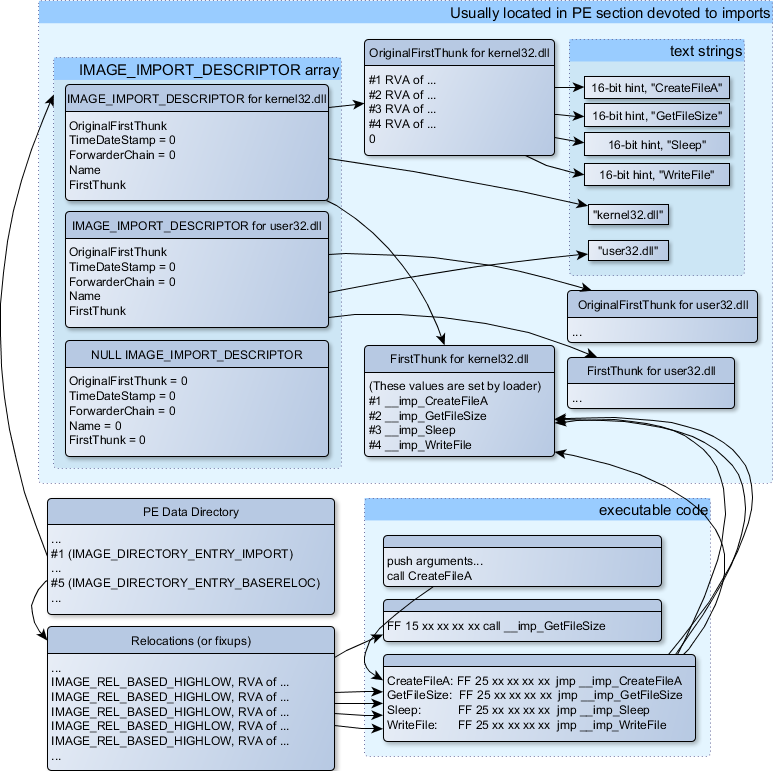
\includegraphics[scale=0.66]{PE/unnamed0.png}
\caption{\IFRU{схема, объеденяющая все структуры в PE-файлы, связанные с импортами}
{The scheme, uniting all PE-file structures related to imports}}
\end{figure}

Самая главная структура, это массив \IT{IMAGE\_IMPORT\_DESCRIPTOR}. Каждый элемент на каждую импортируемую DLL.

У каждого элемента есть \ac{RVA}-адрес текстовой строки-имени DLL (\IT{Name}). \IT{OriginalFirstThink} это \ac{RVA}-адрес
массива \ac{RVA}-адресов, каждый из которых указывает на текстовую строку где записано имя ф-ции, а перед строкой, 
16-битное число (hint) --- ординал ф-ции. Если при загрузке удается найти ф-цию по ординалу, тогда сравнение текстовых
строк не будет происходить. Массив оканчивается нулем. Есть также указатель с названием \IT{FirstThunk}, 
это просто \ac{RVA}-адрес места, где загрузчик будет проставлять адреса найденных ф-ций.

Там, где загрузчик проставляет адреса, \IDA именует их так: \IT{\_\_imp\_CreateFileA}, итд.

Есть по крайней мере два способа обращения к этим полям.

\begin{itemize}
\item
В коде просто указывается \IT{call \_\_imp\_CreateFileA}, а так как, поле с адресом импортируемой ф-ции это
как бы глобальная переменная, то в таблице релоков добавляется адрес в инструкции \IT{call}, 
на случай если модуль будет загружен по другому базовому адресу.

Но как видно, это приводит к увеличению таблицы релоков. Ведь вызовов импортируемой ф-ции у вас в модуле может быть
очень много. К тому же, чем больше таблица релоков, тем дольше загрузка.

\index{thunk-\IFRU{функции}{functions}}
\item
На каждую импортируемую ф-цию выделяется только один переход на импортируемую ф-цию используя инструкцию jmp плюс 
релок на эту инструкцию. Такие места-``переходники'' называются также thunk-ами. 
А все вызовы импортируемой ф-ции это просто инструкция call на ``thunk''. В данном случае, дополнительные релоки
не нужны, потому что эти call-ы имеют относительный адрес, и корректировать их не надо.
\end{itemize}

Оба этих два метода могут комбинироваться. 
Вероятно, линкер создает отдельный ``thunk'', если вызовов слишком много, а по умолчанию --- не создает. \\
\\
Кстати, массив адресов ф-ций, на который указывает FirstThunk, не обязательно может быть в секции импортов.
К примеру, я написал утилиту PE\_add\_import\footnote{\url{http://yurichev.com/PE_add_import.html}} для добавления
импорта в уже существующий .exe-файл. На месте ф-ции, вместо которой вы хотите подставить вызов в другую DLL,
моя утилита вписывает такой код:

\begin{lstlisting}
MOV EAX, [yourdll.dll!function]
JMP EAX
\end{lstlisting}

При этом, FirstThunk указывает прямо на первую инструкцию, т.е., загрузчик, загружая yourdll.dll, прописывает адрес
ф-ции function прямо в коде. Надо также отметить что обычно секция кода защищена от записи, так что, моя утилита
добавляет флаг \IT{IMAGE\_SCN\_MEM\_WRITE} для секции кода, иначе при загрузке такой программы, она упадет с
ошибкой 5 (access denied). \\
\\
Может возникнуть вопрос: а что если я поставляю программу с набором DLL, которые никогда не будут меняться,
может как-то можно ускорить процесс загрузки? Да, можно сразу прописать адреса из DLL в массивы FirstThunk.
Для этого в структуре \IT{IMAGE\_IMPORT\_DESCRIPTOR} имеется поле Timestamp. И если там что-то есть, то загрузчик
сверяет это значение с датой-временем DLL-файла. И если они равны, то он больше ничего не делает, и загрузка будет
происходить быстрее. 
Это называется ``old-style binding''\footnote{\url{http://blogs.msdn.com/b/oldnewthing/archive/2010/03/18/9980802.aspx}. Существует также ``new-style binding'', про него напишу позже}.
В Windows SDK для этого имеется утилита BIND.EXE.
Для ускорения загрузки вашей программы, Matt Pietrek в \cite{Pietrek1}, предлагает делать binding после инсталляции
вашей программы на компьютере конечного пользователя. \\
\\
Запаковщики/зашифровщики PE-файлов могут также сжимать/шифровать секцию импортов. Загрузчик Windows,
конечно же, не загрузит все нужные DLL. Поэтому распаковщик/расшифровщик делает это сам, при помощи
вызовов \IT{LoadLibrary()} и \IT{GetProcAddress()}. \\
\\
В DLL входящих в состав Windows, часто, секция импортов находится в самом начале PE-файла.
Возможно это для оптимизации.
Ведь .exe-файл при загрузке не загружается в память весь (вспомните что инсталляторы огромного размера подозрительно
быстро запускаются), он ``мапится'' (map), и подгружается в память по мере
обращения к этой памяти. И возможно в Microsoft решили что так будет быстрее.

\subsection{Ресурсы}

Ресурсы в PE-файле это набор иконок, картинок, текстовых строк, описаний диалогов.
Возможно, их в свое время решили выделить в отдельное место, чтобы все эти вещи были мультиязычными,
и было проще выбирать текст или картинку того языка, который установлен в \ac{OS}. \\
\\
В качестве побочного эффекта, их легко редактировать и сохранять обратно, даже не обладая специальными знаниями,
например, редактором ResHack\ref{ResHack}.

\subsection{.NET}

\index{.NET}
Программы на .NET компилируются не в машинный код, а в свой собственный байткод.
Собственно, в .exe-файлы байткод вместо обычного кода, однако, точка входа (\ac{OEP}) указывает на крохотный фрагмент
x86-кода:

\begin{lstlisting}
jmp         mscoree.dll!_CorExeMain
\end{lstlisting}

А в mscoree.dll и находится .NET-загрузчик, который уже сам будет работать с PE-файлом.

\index{TLS}
\subsection{TLS}

Эта секция содержит в себе инициализированные данные для \ac{TLS}\ref{TLS} (если нужно). При старте нового треда,
его \ac{TLS}-данные инициализируются данными из этой секции. \\
\\
Помимо всего прочего, спецификация PE-файла предусматривает инициализацию \ac{TLS}-секции, т.н., TLS callbacks.
Если они присутствуют, то они будут вызваны перед тем как передать управление на точку входа (\ac{OEP}).
Это широко используется запаковщиками/защифровщиками PE-файлов.

\subsection{Инструменты}

\begin{itemize}
\item
\index{objdump}
\index{cygwin}
objdump (из cygwin) для вывода всех структур PE-файла

\item
Hiew\ref{Hiew} как редактор

\item
pefile --- Python-библиотека для работы с PE-файлами\footnote{\url{https://code.google.com/p/pefile/}}

\item
\label{ResHack}
ResHack \acs{AKA} Resource Hacker --- редактор ресурсов\footnote{\url{http://www.angusj.com/resourcehacker/}}
\end{itemize}

\subsection{Further reading}

% FIXME: bibliography per chapter or section
\begin{itemize}
\item
Daniel Pistelli --- The .NET File Format \footnote{\url{http://www.codeproject.com/Articles/12585/The-NET-File-Format}}
\end{itemize}

